\section{The affine-plane contraction certificate}
\label{sec:affine}

\subsection{Four geometric plans}
Identify nine group labels with $(x,y)\in\F_3^2$, using integer label
$3x+y$. For each of the four linear forms
\[
 x,\qquad y,\qquad x+y,\qquad x+2y
\]
partition the points into the three level sets. Each set is a line of
three points. Within an ordered line $(a,b,c)$ first merge $b,c$, then
merge the result with $a$. Finally contract the three line tables.
There are six internal merges and one final triangle, hence $21$ support
vectors per plan.

\begin{center}\small
\begin{tabular}{cl}
\toprule Direction & Ordered line blocks\\\midrule
$x$ & $(0,1,2)\mid(3,4,5)\mid(6,7,8)$\\
$y$ & $(0,3,6)\mid(1,4,7)\mid(2,5,8)$\\
$x+y$ & $(0,5,7)\mid(1,3,8)\mid(2,4,6)$\\
$x+2y$ & $(0,4,8)\mid(2,3,7)\mid(1,5,6)$\\
\bottomrule
\end{tabular}\end{center}

\begin{figure}[ht]
\centering
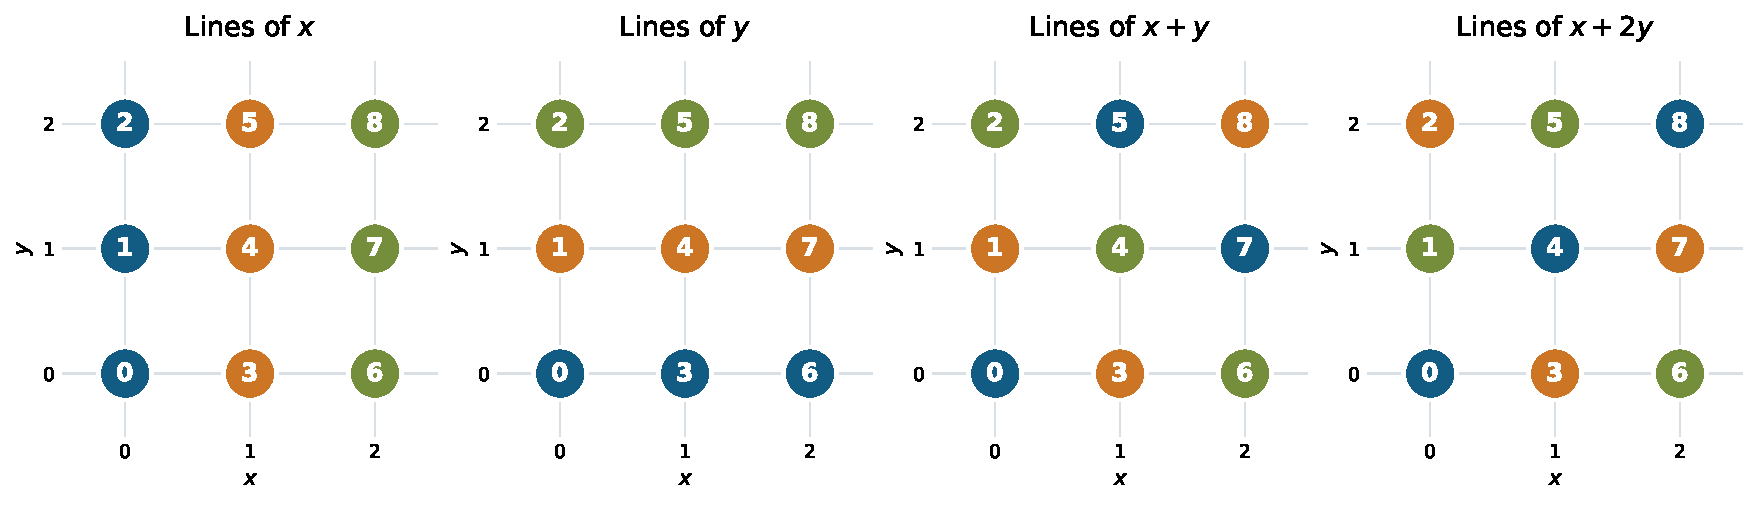
\includegraphics[width=.94\textwidth]{figures/affine_partitions.pdf}
\caption{The same nine groups in four partitions. Equal colors form a
line block. Every pair of distinct points lies together in exactly one
partition, and lines from different partitions meet in one point.}
\end{figure}

These balanced intersection properties are what an arbitrary handful of
permuted trees lacks. They control the overlap between \emph{all} operation
supports, including the operations used to build the tables.

\subsection{A short Gram certificate}
Classify an operation as $P$ (merge two points), $L$ (complete a line), or
$R$ (the root triangle). The following are exact maxima for these four
plans. A transverse pair means supports from different parallel classes.
\begin{center}
\begin{tabular}{crrr}
\toprule Type & $P$ & $L$ & $R$\\\midrule
Maximum single-support squared norm &354&458&486\\
\bottomrule
\end{tabular}\qquad
\begin{tabular}{c|rrr}
Maximum transverse inner product &$P$&$L$&$R$\\\hline
$P$&204&208&215\\
$L$&208&240&260\\
$R$&215&260&288
\end{tabular}
\end{center}
The single-support entries follow directly from the cross-class sizes.
For example, a line-completion operation has undirected class sizes
$2,6,12$, so its largest norm is $4\cdot2+25(6+12)=458$.
A root has three classes of nine edges, giving $9(4+25+25)=486$.
The transverse entries are exact nine-point incidence counts. The
independent checker reconstructs them from Cartesian edge classes.
For the theorem, a short geometric argument supplies slightly weaker
mixed bounds, all still strictly below $288$; no exhaustive computation
is needed for its principal inequality.

A $P$ profile is supported on edges incident to its chosen pair. An $L$
profile is supported on edges incident to its line, except for the edge
between the two points merged first. Transverse lines meet in one point.
Two $P$ supports therefore share at most nine edges, and a $P$ and an
$L$ share at most ten. Since coefficients are at most five, their inner
products are at most $225$ and $250$. In a $P$--$R$ comparison, the
selected points lie in distinct root blocks; eleven root-crossing edges
meet the pair, giving at most $275$.

Two full line-incidence sets share twelve edges: eight incident with their
intersection and four joining their remaining pairs. If the intersection
is not the singleton in at least one of the two line merges, an omitted internal edge is
shared, leaving at most eleven edges and bound $275$. Otherwise the
intersection is the singleton of both merges. Every possible discounted
class contains at least two shared edges; each has product at most ten
instead of twenty-five, so the bound is $300-30=270$.

For $L$--$R$, the transverse line meets each root block once. Root weights
sum to $48$ on its external incident edges and $12$ on its internal
triangle. The line profile omits an internal edge of root weight at least
two, so its undiscounted dot product is at most $5(60-2)=290$.
Its discounted class has root-weight sum at least four, reducing this
by at least $3\cdot4$ to $278$. Thus every mixed transverse inner
product is strictly less than $288$. The root-root case has the exact
geometric proof below. These arguments work for any ordering within a line.

\begin{theorem}[Sharp four-plan certificate]\label{thm:affine}
For the four affine-plane plans,
\[
 \max_{v_j\in\mathcal V_j}\left\|v_1+v_2+v_3+v_4\right\|_2^2=5400.
\]
Consequently their local coefficient in Lemma~\ref{lem:certificate} is
$\beta_9=1/\sqrt3$.
\end{theorem}
\begin{proof}
The Gram bounds give
\[
 \left\|\sum_jv_j\right\|_2^2
 =\sum_j\|v_j\|_2^2+2\sum_{j<k}\langle v_j,v_k\rangle
 \le4\cdot486+2\binom42\,288=5400.
\]
Every choice of four root supports attains equality. Here is a geometric
verification, also explaining why the constant is simple.
Let $C_j$ be the cross-edge set of direction $j$ and let $D_j$ join the
two parallel lines chosen for its discounted class. A root support is
$5\mathbf1_{C_j}-3\mathbf1_{D_j}$. For distinct directions,
\[
 |C_j\cap C_k|=18,\quad |D_j\cap C_k|=|C_j\cap D_k|=6,
 \quad |D_j\cap D_k|=2.
\]
The last identity counts the two diagonals of the affine $2$ by $2$
rectangle obtained by retaining two levels of each independent linear
form. Therefore every transverse root inner product is
$25\cdot18-15(6+6)+9\cdot2=288$. Each root norm is $486$.
Finally
\[
 \beta_9^2=\frac{2\cdot5400}{25\cdot4^2\cdot9^2}=\frac13.
\]
\end{proof}

As an additional independent check, all $21^4=194{,}481$ tuples were
enumerated with integer arithmetic. The sum of their squared norms is
$622{,}974{,}240$. Exactly $81=3^4$ tuples attain $5400$; every one
uses four root supports. The largest value involving an internal operation
is $5204$. These checks support the finite incidence table; they are not
samples of entropy vectors.

\subsection{Sharpness within this particular menu}
The coefficient is the exact minimax value for this four-plan support
model, not merely a convenient sufficient bound. Choose any root support
$v_j$ from each direction and set $g=\sum_jv_j$. Then
$\|g\|_2^2=5400$ and
\[
 v_j\cdot g=486+3\cdot288=1350\qquad(1\le j\le4).
\]
Thus every plan has $F_j(g)\ge270$. The averaging bound gives equality.
Assigning each directed orientation half the corresponding $g_e$ and
normalizing to the Euclidean entropy ball witnesses the coefficient
$1/\sqrt3$. This is not an optimality claim over all possible tree menus,
over actual realizable mode lists, or over SAT algorithms.

\subsection{A second finite certificate for the recursive bottleneck}
For thirteen groups use the following four plans. In each block, recursively
split the ordered list at its floor midpoint, build the two subblocks, and
merge. Finish with the three-block triangle.
\begin{center}\small
\begin{tabular}{cl}
\toprule Plan & Ordered blocks\\\midrule
1 & $(0,1,2,3,4)\mid(5,6,7,8)\mid(9,10,11,12)$\\
2 & $(12,10,1,6,4)\mid(9,0,3,8)\mid(5,2,7,11)$\\
3 & $(0,8,11,12,1)\mid(7,10,4,3)\mid(5,2,6,9)$\\
4 & $(1,7,0,6,9)\mid(5,10,11,3)\mid(12,8,4,2)$\\
\bottomrule
\end{tabular}\end{center}
The first three plans occur in the incoming certificate; adding the fourth
and certifying the complete new menu is the additional finite refinement.
There are eleven operations and $33$ profiles per plan. Direct exact
evaluation gives squared norm at most $1064$ for every single profile
and inner product at most $647$ for every pair from different plans.
Consequently
\[
 Q_{13}\le4\cdot1064+12\cdot647=12020,
 \qquad \beta_{13}^2=\frac{2\cdot12020}{25\cdot16\cdot169}
 =\frac{601}{1690}.
\]
Equality occurs when each final triangle discounts the class between its
two four-point blocks. The $6534=6\cdot33^2$ pairwise integer checks
and the matching witness suffice to certify this bound. Two independently
written programs also enumerate all $33^4=1{,}185{,}921$ tuples;
their squared-norm sum is $5{,}700{,}575{,}232$, with a unique maximizer.
No floating search result is used as a mathematical acceptance condition.

For completeness, the finite Gram calculation is exactly the following:
\begin{lstlisting}
for plan in plans:
    operations = binary_merges_inside_blocks(plan) + [final_triangle(plan)]
    profiles = [cross_class_weights(op, discount, high=5, low=2)
                for op in operations for discount in range(3)]
check(all(dot(v,v) <= 1064 for v in every_profile))
check(all(dot(v,w) <= 647 for v,w in different_plan_pairs))
check(dot(sum_of_four_displayed_root_profiles,
          sum_of_four_displayed_root_profiles) == 12020)
\end{lstlisting}
The supplied plans, midpoint rule, pair coordinates, and profile definition
fully specify this finite certificate.

\subsection{Why a better local bound is not enough}
The incoming best cached schedule has its maximum at the second recursion
stage, not at the root. Replacing its nine-group coefficient alone would
improve memory but leave the time coefficient $30.8910189\ldots$ unchanged.
The global construction must also improve that later bottleneck. The next
section includes the needed second certificate, its actual child-entry
costs, and an explicit feasible schedule. This prevents a local-only gain
from being reported as a global speedup.
